% ED-18 -- Fixation probabilities as absorption limits, kernel-checked (Wright-Fisher, Moran, Price)
% English translation of papers/discovery_journal_2026/chapters/c06.tex
% Sources: TOP20.json pick 6; papers/prog_population_genetics_fixation/{AUDIT.md,REVISION.md,publication_meta.json}
% Figure: code/fig06.py -> figures/c06_fixation.{pdf,png}
\chapter[A mutation's chance of taking over]{What chance does a mutation have of taking over a population?}
\reference{Preprint of 25 October 2026, published 26 October 2026.\\ doi:10.5281/\\zenodo.23653850}

\section*{The idea in one picture}

\begin{analogie}
Imagine a token placed on a ladder of $N+1$ rungs, numbered from $0$ to $N$. The number of the rung is the number
of carriers of a new mutation in a population of $N$ individuals. At each turn we roll a loaded die: the token
goes up one rung, goes down one rung, or stays where it is. Both ends are traps: at rung~$0$ the mutation has
disappeared, at rung~$N$ it has taken over everyone, and the game stops. The question is: starting from rung~$i$,
what is the chance of ending at the top? This chapter tells how this classic calculation was redone, with every
line checked by a tireless referee, a program.

\emph{Where the picture stops being accurate:} in the Wright--Fisher model the token can jump several rungs at
once, and a real population has neither a fixed size nor an unchanging die; the referee checks the calculation
on the model, not that the model describes nature.
\end{analogie}

\section*{What was done}

Population geneticists have long known the answer for two textbook models. In the \emph{Moran} model, at each step
one individual is chosen to reproduce, with a chance proportional to its ``fitness'' (the mutant is worth $r$, the
others are worth~$1$), and its offspring replaces an individual picked at random. In the \emph{Wright--Fisher}
model, the whole generation is renewed at once by random sampling. With no advantage ($r=1$), in both models the
chance of taking over, starting from $i$ mutants, is simply $i/N$. In the Moran model, with an advantage $r$, it is
\[
\rho(i)=\frac{1-r^{-i}}{1-r^{-N}} .
\]

This work proves these formulas in Lean, a proof assistant whose small core, called the \emph{kernel}, rejects any
step that does not follow strictly from the previous ones. The proof does not talk about chance in a vague sense:
it takes the table of one-step probabilities (a matrix $P$), computes what happens after $n$ steps (the power
$P^n$), and proves that the ``top'' entry of this table converges to $\rho(i)$ as $n$ grows. A single general
theorem covers both models. It requires one condition: in the middle of the ladder, the token must keep real
uncertainty at every step (a positive ``variance''). The same work also proves the Price equation, an exact
identity about how the average of a trait changes in a finite population, and a simple special case that follows
from it.

\begin{encadre}
\textbf{To do with a pencil.} Take $N=2$ individuals, a single mutant ($i=1$) that reproduces twice as often
($r=2$). The total weight is $2+1=3$.
\begin{itemize}
\item The token goes up if the mutant is chosen (chance $2/3$) and its offspring replaces the other individual
  (chance $1/2$): $2/3\times1/2=1/3$.
\item It goes down if the other individual is chosen ($1/3$) and replaces the mutant ($1/2$): $1/6$.
\item It stays in place the rest of the time: $1-1/3-1/6=1/2$.
\end{itemize}
Call $h$ the chance of taking over from rung~$1$. After one turn, we have either won (chance $1/3$), lost (chance
$1/6$), or come back to the starting point (chance $1/2$): $h=1/3+\tfrac12 h$, so $h=2/3$. The formula indeed gives
$(1-1/2)/(1-1/4)=(1/2)/(3/4)=2/3$. With three individuals, it gives $(1-1/2)/(1-1/8)=4/7\approx0.571$, against
$1/3$ with no advantage. Figure~\ref{fig:c06} shows, turn after turn, the probability of having already taken over
climbing towards this $4/7$.
\end{encadre}

In parallel, a new module of the numerical solver rusty-SUNDIALS (a translation into Rust of the CVODE solver)
handled the continuous-time version of these chains behind a ``certificate'' that rejects any doubtful result.
Over 106 accepted computations, the gap to the exact formulas never exceeds $3.1\times10^{-10}$, and the 9
counter-tests deliberately rigged (inverted exponent, neutral value under selection, a matrix that never moves,
a duration that is too short, a corrupted row) were all rejected.

\begin{figure}[htbp]
\centering
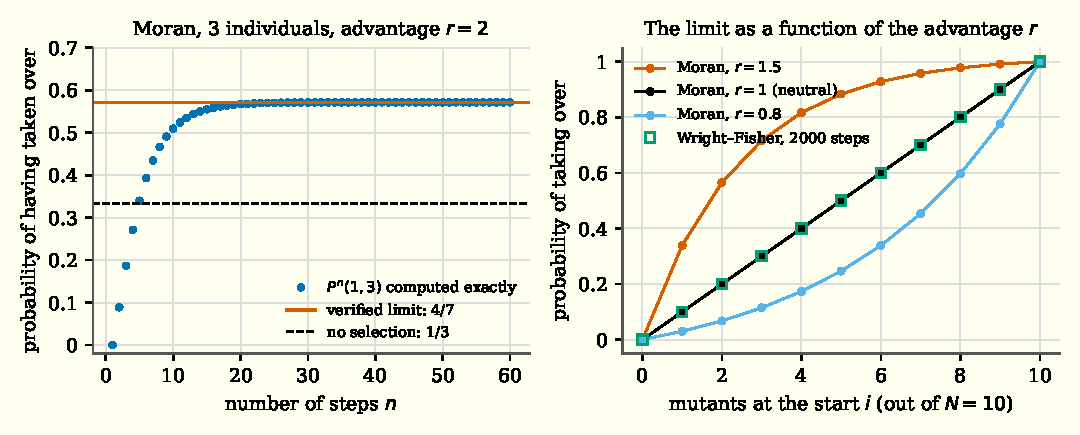
\includegraphics[width=\linewidth]{figures/c06_fixation}
\caption{Probability of having taken over after $n$ steps (left); final chance according to the advantage $r$ (right).}
\label{fig:c06}
\end{figure}

\section*{How we made sure it is not wrong}

In short: \niveau{A} for the statements about matrix powers, \niveau{C} for their reading in terms of trajectories,
\niveau{X} for the simulation.

For the proved statements, ``the judge has looked'': the Lean kernel checked every step, and the only starting
assumptions allowed (the ``axioms'') stay within a short whitelist of three standard principles. An AI agent
distinct from the one that produced the work, but from the same family of models, rebuilt everything from the
sources in its own directory: the 14 level-A statements pass again. It also planted traps, which were meant to
fail and did fail:
\begin{itemize}
\item a ``proof'' of a false limit, plugged with a hole (\texttt{sorry}) or with an invented axiom: the file still
  compiles without error, but the axiom audit flags the cheat;
\item the verified value $4/7$ replaced by $1/3$: the kernel refuses.
\end{itemize}
One counter-test lives inside the theorems themselves: a chain that does have its two trap ends and a consistent
arrival function, but is never absorbed. It shows that the variance condition is not decorative. The auditor
redid the numerical computation and obtained a file identical byte for byte, and the complete replay of the
proofs in the kernel, on 26 October 2026, passed without error. The claims register nevertheless remains at
``unaudited'': no human has yet checked that the Lean statements really say what their plain-language summaries
announce.

\section*{What this does not say}

\begin{limite}
\begin{itemize}
\item Nothing new in biology: these are textbook results, and the work claims no priority. What is new is that a
  checker has verified them, and that the building blocks are reusable.
\item The kernel verified limits of matrix powers. That these are ``the probability of reaching $N$ before time
  $n$'' is the standard definition, but this link is not formalized (\niveau{C}).
\item One objective announced in advance, Fisher's fundamental theorem in its general form, \emph{was not
  reached}; only a simple special case is proved.
\item The CVODE computations are a sketch \niveau{X}: they illustrate, they prove nothing.
\item The original papers of 1958, 1970 and 1972 were not read directly, which the article says itself.
\end{itemize}
\end{limite}

\section*{Going further}

The article, its register and the audit are deposited under doi:10.5281/\allowbreak zenodo.23653850. The
``absorption'' and ``Moran model'' building blocks are reused as they are by the work on the isothermal theorem,
which moves from the well-mixed population to a population placed on a network (doi:10.5281/zenodo.23660071).
